\documentclass[tikz]{standalone}
\usetikzlibrary{positioning}

\begin{document}
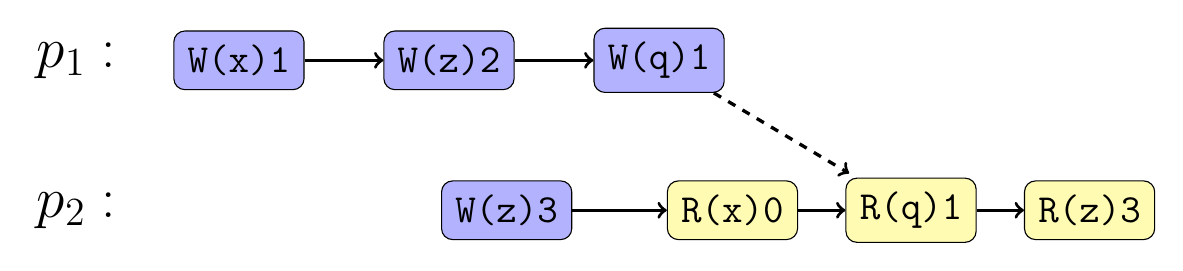
\begin{tikzpicture}
\tikzset{
  wop/.style = {rectangle, rounded corners, fill = blue!30, draw, font = \Large, inner sep = 5pt},
  rop/.style = {rectangle, rounded corners, fill = yellow!30, draw, font = \Large, inner sep = 5pt}, process/.style = {font = \huge}, po/.style = {->, very thick},
  rw/.style = {->, shorten >= 3pt, very thick, dashed},
  vis/.style = {->, shorten >= 3pt, very thick, dashed}
}

  \node (p1) [process] {$p_1:$};
  \node (wx1) [wop, right = 0.6cm of p1] {\texttt{W(x)1}};
  \node (wz2) [wop, right = 1cm of wx1] {\texttt{W(z)2}};
  \node (wq1) [wop, right = 1cm of wz2] {\texttt{W(q)1}};

  \node (p2) [process, below = 1.2cm of p1] {$p_2:$};
  \node (wz3) [wop, right = 4cm of p2] {\texttt{W(z)3}};
  \node (rx0) [rop, right = 1.2cm of wz3] {\texttt{R(x)0}};
  \node (rq1) [rop, right = 0.6cm of rx0] {\texttt{R(q)1}};
  \node (rz3) [rop, right = 0.6cm of rq1] {\texttt{R(z)3}};

  \draw [po] (wx1) to (wz2);
  \draw [po] (wz2) to (wq1);

  \draw [po] (wz3) to (rx0);
  \draw [po] (rx0) to (rq1);
  \draw [po] (rq1) to (rz3);

  \draw [vis] (wq1) to (rq1);

\end{tikzpicture}
\end{document}
